\documentclass[dvipsnames]{beamer}

\usetheme{Frankfurt}
\usecolortheme{dove}
\setbeamertemplate{navigation symbols}{}
\setbeamertemplate{itemize items}[circle]
\usefonttheme{professionalfonts}

\usepackage[utf8]{inputenc}
\usepackage[T1]{fontenc}
\usepackage{lmodern}

\usepackage{amsmath}
\usepackage{amssymb}
\usepackage{amsfonts}
\usepackage{bm}
\usepackage{float}
\usepackage{subcaption}
\usepackage{graphicx}
\usepackage{tabulary}
\usepackage{longtable}
\usepackage{siunitx}

% \usepackage[]{xcolor}
\usepackage{tikz}
\usetikzlibrary{arrows,decorations.pathmorphing,backgrounds,positioning,fit,petri,decorations.pathreplacing}
\tikzset{circly/.style={draw,circle,minimum size=1cm},
    arraycell/.style={draw,rectangle,minimum size=1cm,node distance=0},
    accolade/.style={decorate,decoration={brace,amplitude=10pt}},
    enoughdamnvspace/.style={font=\vphantom{$ f $}},
    smallnode/.style={circle,fill,inner sep=0,minimum size=5pt}
}
\usepackage{pgfplots, pgfplotstable}
\pgfplotsset{compat=1.16}
\pgfplotsset{legend style={fill opacity=0.7,text opacity=1}}
\pgfplotsset{cycle list={
    {thick,MidnightBlue,mark=*},
    {mark options=solid,dashed,thick,OrangeRed,mark=square*},
    {thick,YellowOrange,mark=diamond*},
    {thick,Fuchsia,mark=asterisk},
    {mark options=solid,dashed,thick,ForestGreen,mark=x},
    {thick,Turquoise,mark=square*},
    {Black,mark=triangle*},
    {mark options=solid,dashed,thick,RedViolet,mark=diamond*},
    {LimeGreen,mark=square*}
}}
\pgfplotsset{axis lines=left}

\usepackage{algorithm}
\usepackage{algorithmicx}
\usepackage[noend]{algpseudocode}

\renewcommand{\sfdefault}{phv}
\renewcommand{\rmdefault}{bch}
\def\mytablesize{\small}

\algnewcommand{\LineComment}[1]{\State \(/*\) #1 \(*/\)}

\frenchspacing


\newcommand{\sequencetickmarks}[3]
{
% args: (number of tick marks, x of first tick mark, y of first tick mark)
    \pgfmathsetmacro\secondtickmark{#2+0.5}
    \pgfmathsetmacro\lasttickmark{#2+0.5*#1}

    \draw (#2,#3) -- (\lasttickmark,#3);

    \foreach \x in {#2,\secondtickmark,...,\lasttickmark}
        \draw (\x,#3) -- +(0,3pt);
}

\newcommand{\sequenceeventtypes}[4]
{
% args: (x of first event, y, t of first event, list of t/A pairs)
    \pgfmathsetlengthmacro\nodeheight{(#2)+(.8em)}

    \foreach \t/\eventtype [evaluate=\t as \x using (\t-#3)*0.5+(#1)] in {#4}
    {
        \node [font=\vphantom{$ fbd $}] at (\x,#2) {$ \eventtype $};
        \node (t\t) [inner sep=0] at (\x,\nodeheight) {};
    }
}

\newcommand{\windowthingy}[2]
{
% args: starting position (leftmost point of horizontal line), number of timestamps
    \pgfmathsetmacro\windowthingylength{#2*0.5-0.1}
    \draw [thick] #1 ++(0,3pt) -- ++(0,-3pt) -- ++(\windowthingylength,0) -- ++(0,3pt);
}

\newcommand{\examplesequence}
{
    \sequencetickmarks{23}{-5.5}{0}

    \sequenceeventtypes{-5.5}{1em}{30}{32/c,33/f,34/b,35/b,38/c,40/d,41/a,44/b,46/e,47/a,48/e,49/c};
}

\newcommand{\examplesequencetimestamps}
{
    \foreach \x [evaluate=\x as \timestamp using int((\x*2)+41)] in {-5.5,-3,...,5.5}
    \node at (\x,-1em) {$ \timestamp $};
}

\begin{document}

\title{Evaluation of Algorithms for Sequential Pattern Mining in Long Event Sequences}
\author{Josse Coen}
\date{6 September 2018}

\frame{\titlepage}

\begin{frame}
\frametitle{Goal}

\begin{itemize}
\item Can we find interesting patterns in event sequences?
\item Can we do so efficiently?
\end{itemize}

\end{frame}
\begin{frame}
\frametitle{Event sequences}

\begin{align*}
\Sigma = \{ a, b, c, d, e, f \}
\end{align*}

\begin{center}
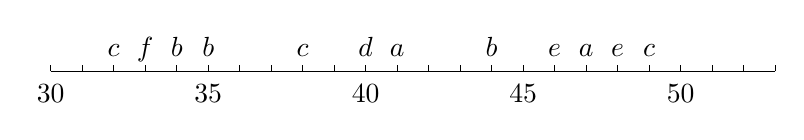
\begin{tikzpicture}[scale=0.8]

\examplesequence
\examplesequencetimestamps

\end{tikzpicture}
\end{center}

\end{frame}
\begin{frame}
\frametitle{Window on a sequence}

\begin{center}
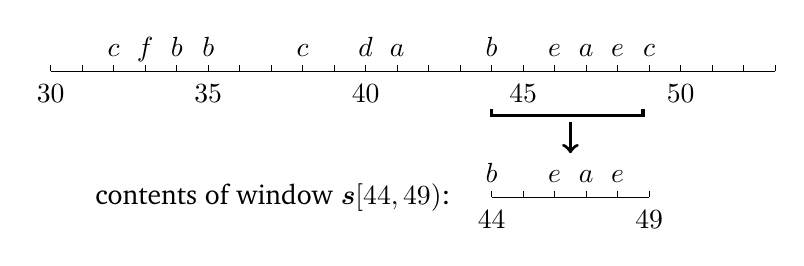
\begin{tikzpicture}[scale=0.8]

\examplesequence
\examplesequencetimestamps

\draw [very thick] (1.5,-0.6) -- ++(0,-3pt) -- ++(2.4,0) -- ++(0,3pt);

\draw [->,very thick] (2.75,-0.8) -- ++(0,-0.5);

\draw (1.5,-2) -- ++(2.5,0);

\foreach \x in {1.5,2,...,4}
    \draw (\x,-2) -- ++(0,3pt);

\foreach \x/\label in {
    1.5/b,
    2.5/e,
    3/a,
    3.5/e}
    \path (\x,-2) ++(0,1em) node [enoughdamnvspace] {$ \label $};

\path (1.5,-2) ++(0,-1em) node {$ 44 $};
\path (4,-2) ++(0,-1em) node {$ 49 $};

\node [anchor=east] at (1,-2) {contents of window $ \boldsymbol{s}[44,49) $:};

\end{tikzpicture}
\end{center}

\end{frame}
\begin{frame}
\frametitle{Episodes}

labelled directed acyclic graph

\begin{align*}\alpha=(V, E, lab)\end{align*}

\begin{itemize}
\item $ (V, E) $ directed acyclic graph
\item $ lab : V \to \Sigma $ mapping of nodes to event types
\end{itemize}

\end{frame}
\begin{frame}
\frametitle{Parallel episodes}

\begin{itemize}
\item all episodes $ (V, E, lab) $ for which $ E = \emptyset $
\item notation: \begin{align*} \{ A_1, A_2, \ldots, A_n \} \end{align*} with $ A_i $ event types
\end{itemize}

\end{frame}
\begin{frame}
\large
\begin{center}
\begin{tikzpicture}[scale=1.5]
\node (parB) at (3,2.6) [smallnode,label={$ b $}] {};
\node (parE1) at (2,1.8) [smallnode,label={$ e $}] {};
\node (parE2) at (4.5,2.4) [smallnode,label={$ e $}] {};
\node (parC) at (3.5,2) [smallnode,label={$ c $}] {};
\end{tikzpicture}
\end{center}

\end{frame}
\begin{frame}
\frametitle{Serial episodes}

\begin{itemize}
\item all episodes $ (V, E, lab) $ for which $ E $ defines total order on $ V $
\item notation: \begin{align*} A_1 \to A_2 \to \cdots \to A_n \end{align*} with $ A_i $ event types
\end{itemize}

\end{frame}
\begin{frame}
\large
\begin{center}
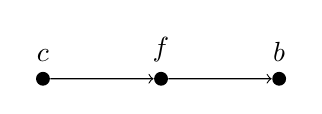
\begin{tikzpicture}[scale=1.5]
\node (serC) at (-5,2.5) [smallnode,label={$ c $}] {};
\node (serF) at (-4,2.5) [smallnode,label={$ f $}] {};
\node (serB) at (-3,2.5) [smallnode,label={$ b $}] {};

\draw [->] (serC) -- (serF);
\draw [->] (serF) -- (serB);
\end{tikzpicture}
\end{center}

\end{frame}
\begin{frame}
\frametitle{Occurrences}

\begin{center}
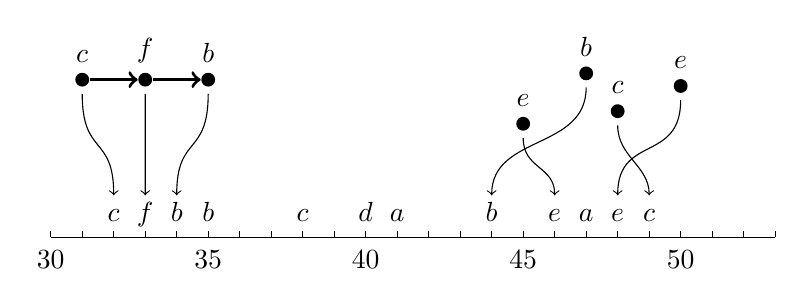
\begin{tikzpicture}[scale=0.8]

\examplesequence
\examplesequencetimestamps

% serial episode

\node (serC) at (-5,2.5) [smallnode,label={$ c $}] {};
\node (serF) at (-4,2.5) [smallnode,label={$ f $}] {};
\node (serB) at (-3,2.5) [smallnode,label={$ b $}] {};

\draw [->,very thick] (serC) -- (serF);
\draw [->,very thick] (serF) -- (serB);

\draw [->] ([yshift=-3pt]serC.south) .. controls +(0,-1) and +(0,1) .. (t32);
\draw [->] ([yshift=-3pt]serF.south) .. controls +(0,-1) and +(0,1) .. (t33);
\draw [->] ([yshift=-3pt]serB.south) .. controls +(0,-1) and +(0,1) .. (t34);

% parallel episode

\node (parB) at (3,2.6) [smallnode,label={$ b $}] {};
\node (parE1) at (2,1.8) [smallnode,label={$ e $}] {};
\node (parE2) at (4.5,2.4) [smallnode,label={$ e $}] {};
\node (parC) at (3.5,2) [smallnode,label={$ c $}] {};

\draw [->] ([yshift=-3pt]parB.south) .. controls +(0,-1) and +(0,1) .. (t44);
\draw [->] ([yshift=-3pt]parE1.south) .. controls +(0,-0.5) and +(0,0.5) .. (t46);
\draw [->] ([yshift=-3pt]parE2.south) .. controls +(0,-1) and +(0,1) .. (t48);
\draw [->] ([yshift=-3pt]parC.south) .. controls +(0,-0.5) and +(0,0.5) .. (t49);

\end{tikzpicture}
\end{center}

\end{frame}
% TODO include this?
\iffalse
\begin{frame}
\frametitle{Parallel episodes: array representation}

\begin{center}
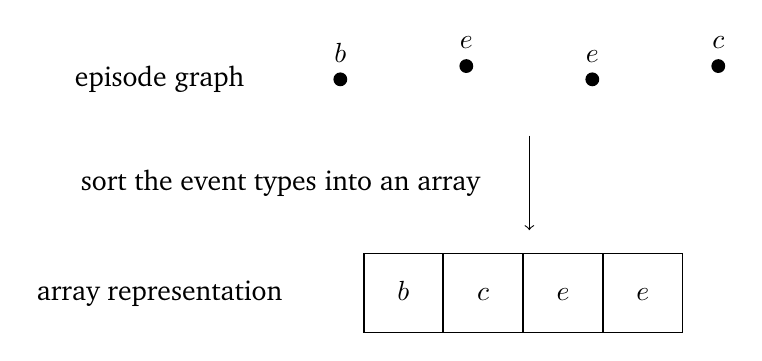
\begin{tikzpicture}[scale=0.8]

\node (n 1) [smallnode,label=above:$ b $] at (-3,-3pt) {};
\node (n 2) [smallnode,label=above:$ e $] at (-1, 3pt) {};
\node (n 3) [smallnode,label=above:$ e $] at ( 1,-3pt) {};
\node (n 4) [smallnode,label=above:$ c $] at ( 3, 3pt) {};

\node (episodegraphtext) [left=of n 1] {episode graph};

\draw [->] (0,-1) -- node [left=0.5cm] {sort the event types into an array} +(0,-1.5);

\node (a 1) [arraycell,enoughdamnvspace] at (-2,-3.5) {$ b $};
\node (a 2) [arraycell,right=of a 1,enoughdamnvspace] {$ c $};
\node (a 3) [arraycell,right=of a 2,enoughdamnvspace] {$ e $};
\node (a 4) [arraycell,right=of a 3,enoughdamnvspace] {$ e $};

\node at (episodegraphtext |- a 1) {array representation};

\end{tikzpicture}
\end{center}

\end{frame}
\begin{frame}
\frametitle{Serial episodes: array representation}

\begin{center}
\begin{tikzpicture}[scale=0.8]

\node (n 1) [smallnode,label=above:$ c $] at (-3,0) {};
\node (n 2) [smallnode,label=above:$ f $] at (-1,0) {}
    edge [pre] (n 1);
\node (n 3) [smallnode,label=above:$ b $] at (1, 0) {}
    edge [pre] (n 2);
\node (n 4) [smallnode,label=above:$ b $] at (3, 0) {}
    edge [pre] (n 3);

\node [left=of n 1] {episode graph};

\draw [->] (0,-1) -- node [left=0.5cm,align=right] {store event types into array,\\preserving topological ordering} +(0,-1.5);

\node (a 1) [arraycell,enoughdamnvspace] at (-2, -3.5) {$ c $};
\node (a 2) [arraycell,right=of a 1,enoughdamnvspace] {$ f $};
\node (a 3) [arraycell,right=of a 2,enoughdamnvspace] {$ b $};
\node (a 4) [arraycell,right=of a 3,enoughdamnvspace] {$ b $};

\node at (episodegraphtext |- a 1) {array representation};

\end{tikzpicture}
\end{center}

\end{frame}
\fi
\begin{frame}
\frametitle{Subepisode relationship}

\begin{align*}
\alpha \subseteq \beta \iff \text{ all sequences that cover } \beta \text{ also cover } \alpha
\end{align*}

\end{frame}
\begin{frame}
\frametitle{Interestingness measures for episodes}
% TODO introduce interestingness measures, frequency measures in particular, monotonicity and why necessary

Two main interpretations:

\begin{itemize}
\item \textbf{frequency}: how often does an episode occur?
\item \textbf{cohesion}: how close together are events that constitute occurrences?
\end{itemize}

\end{frame}
\begin{frame}
\frametitle{High-level episode mining procedure}

\begin{algorithmic}[1]

\State $ \mathcal{C}_1 \gets \{ \langle A \rangle \mid A \in \Sigma \} $
\State $ l \gets 1 $
\While{$ \mathcal{C}_l \neq \emptyset $}
    \LineComment{Database pass}
    \State $ \mathcal{F}_l \gets \{ \alpha \in \mathcal{C}_l \mid fr_\Psi(\alpha, \boldsymbol{s}, \rho) \geq \text{min\_fr} \} $
    \State $ l \gets l + 1 $
    \LineComment{Candidate generation}
    \State $ \mathcal{C}_l \gets \{ \alpha \mid | \alpha | = l \wedge \forall \beta \mid \beta \subset \alpha : fr_\Psi(\beta, \boldsymbol{s}, \rho) \geq \text{min\_fr} \} $
\EndWhile
\ForAll{$ i \mid | \mathcal{F}_i | > 0 $}
    \State output $ \mathcal{F}_i $
\EndFor

\end{algorithmic}

\end{frame}
\begin{frame}
% candidate generation figure

\begin{center}
\begin{tikzpicture}

\newcommand{\sharedprefix}[1]{\ifcase####1 a\or a\or b\fi}

\foreach \arrayindex [evaluate=\arrayindex as \leftx using int(\arrayindex-4),
                      evaluate=\arrayindex as \rightx using (int(\arrayindex+1))] in {0,...,2}
{
    \node (n\arrayindex0) [arraycell,enoughdamnvspace] at (\leftx,0.75) {$ \sharedprefix{\arrayindex} $};
    \node (n\arrayindex1) [arraycell,enoughdamnvspace] at (\leftx,-0.75) {$ \sharedprefix{\arrayindex} $};
    \node (n\arrayindex2) [arraycell,enoughdamnvspace] at (\rightx,0) {$ \sharedprefix{\arrayindex} $};
}

\node (n30) [arraycell,enoughdamnvspace,color=OrangeRed] at (-1,0.75) {$ b $};
\node (n31) [arraycell,enoughdamnvspace,color=MidnightBlue] at (-1,-0.75) {$ c $};

\node (n32) [arraycell,enoughdamnvspace,color=OrangeRed] at (4,0) {$ b $};
\node (n42) [arraycell,enoughdamnvspace,color=MidnightBlue] at (5,0) {$ c $};

\draw [->] (n30.north) to [bend left=45] (n32.north);
\draw [->] (n31.south) to [bend right=45] (n42.south);

\draw [accolade] (n21.south east) -- node (acc1tip) [inner sep=0,midway,yshift=-10pt] {} (n01.south west);
\draw [accolade] (n22.south east) -- node (acc2tip) [inner sep=0,midway,below,yshift=-10pt] {} (n02.south west);

\draw [->] (acc1tip) to [bend right=45] (acc2tip);

% \node [above=of n00] {first episode};
% \node [below=of n01] {second episode};

% \node [right=5pt of n42] {potential candidate};

\end{tikzpicture}
\end{center}

\end{frame}
\begin{frame}
\begin{center}
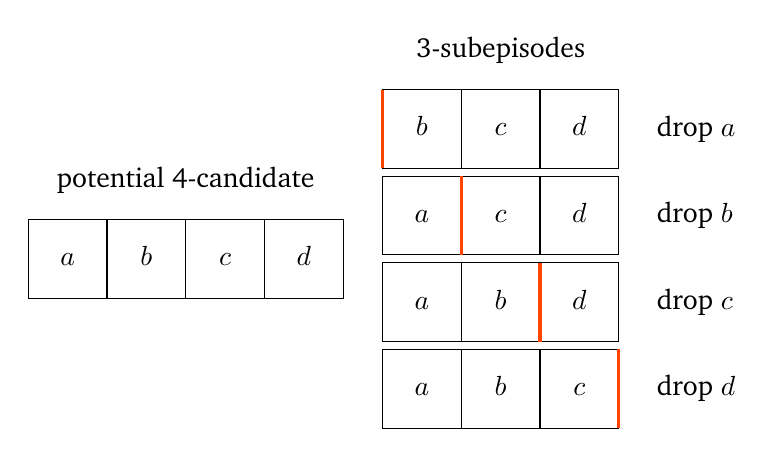
\begin{tikzpicture}

\node at (2,1) {potential 4-candidate};
\node at (6,2.65) {3-subepisodes};

\node [arraycell,enoughdamnvspace] at (0.5,0) {$ a $};
\node [arraycell,enoughdamnvspace] at (1.5,0) {$ b $};
\node [arraycell,enoughdamnvspace] at (2.5,0) {$ c $};
\node [arraycell,enoughdamnvspace] at (3.5,0) {$ d $};

\node [arraycell,enoughdamnvspace] at (5,1.65) {$ b $};
\node [arraycell,enoughdamnvspace] at (6,1.65) {$ c $};
\node (r0) [arraycell,enoughdamnvspace] at (7,1.65) {$ d $};
\node [right=10pt of r0] {drop $ a $};
\draw [OrangeRed,very thick] (4.5,2.15) -- ++(0,-1);

\node [arraycell,enoughdamnvspace] at (5,0.55) {$ a $};
\node [arraycell,enoughdamnvspace] at (6,0.55) {$ c $};
\node (r1) [arraycell,enoughdamnvspace] at (7,0.55) {$ d $};
\node [right=10pt of r1] {drop $ b $};
\draw [OrangeRed,very thick] (5.5,1.05) -- ++(0,-1);

\node [arraycell,enoughdamnvspace] at (5,-0.55) {$ a $};
\node [arraycell,enoughdamnvspace] at (6,-0.55) {$ b $};
\node (r2) [arraycell,enoughdamnvspace] at (7,-0.55) {$ d $};
\node (dropC) [right=10pt of r2] {drop $ c $};
\draw [OrangeRed,very thick] (6.5,-0.05) -- ++(0,-1);

\node [arraycell,enoughdamnvspace] at (5,-1.65) {$ a $};
\node [arraycell,enoughdamnvspace] at (6,-1.65) {$ b $};
\node (r3) [arraycell,enoughdamnvspace] at (7,-1.65) {$ c $};
\node (dropD) [right=10pt of r3] {drop $ d $};
\draw [OrangeRed,very thick] (7.5,-1.15) -- ++(0,-1);

% \draw [accolade] ([xshift=-2pt]dropC.east |- r2.north) -- node [midway,right,align=left,xshift=12pt] {last two are frequent\\since candidate was\\built upon them} ([xshift=-2pt]dropD.east |- r3.south);

\end{tikzpicture}
\end{center}
\end{frame}
\begin{frame}
\frametitle{Fixed-window frequency}

The fixed-window frequency is defined as the number of fixed-width windows that cover $ \alpha $.
\begin{align*}
fr_f(\alpha) = | \{ \boldsymbol{s}[t, t + \rho) \mid \boldsymbol{s}[t, t + \rho) \text{ covers } \alpha \} |
\end{align*}

for a given window width $ \rho $, sequence $ \boldsymbol{s} $.

\end{frame}
\begin{frame}
\begin{center}
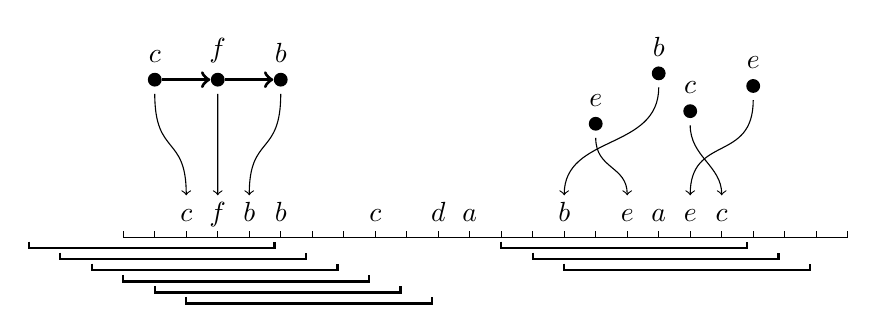
\begin{tikzpicture}[scale=0.8]

\examplesequence

%% draw occurrence proofs again
% serial episode

\node (serC) at (-5,2.5) [smallnode,label={$ c $}] {};
\node (serF) at (-4,2.5) [smallnode,label={$ f $}] {};
\node (serB) at (-3,2.5) [smallnode,label={$ b $}] {};

\draw [->,very thick] (serC) -- (serF);
\draw [->,very thick] (serF) -- (serB);

\draw [->] ([yshift=-3pt]serC.south) .. controls +(0,-1) and +(0,1) .. (t32);
\draw [->] ([yshift=-3pt]serF.south) .. controls +(0,-1) and +(0,1) .. (t33);
\draw [->] ([yshift=-3pt]serB.south) .. controls +(0,-1) and +(0,1) .. (t34);

% parallel episode

\node (parB) at (3,2.6) [smallnode,label={$ b $}] {};
\node (parE1) at (2,1.8) [smallnode,label={$ e $}] {};
\node (parE2) at (4.5,2.4) [smallnode,label={$ e $}] {};
\node (parC) at (3.5,2) [smallnode,label={$ c $}] {};

\draw [->] ([yshift=-3pt]parB.south) .. controls +(0,-1) and +(0,1) .. (t44);
\draw [->] ([yshift=-3pt]parE1.south) .. controls +(0,-0.5) and +(0,0.5) .. (t46);
\draw [->] ([yshift=-3pt]parE2.south) .. controls +(0,-1) and +(0,1) .. (t48);
\draw [->] ([yshift=-3pt]parC.south) .. controls +(0,-0.5) and +(0,0.5) .. (t49);

% windows

\windowthingy{(-7,-5pt)}{8}
\windowthingy{(-6.5,-10pt)}{8}
\windowthingy{(-6,-15pt)}{8}
\windowthingy{(-5.5,-20pt)}{8}
\windowthingy{(-5,-25pt)}{8}
\windowthingy{(-4.5,-30pt)}{8}

\windowthingy{(0.5,-5pt)}{8}
\windowthingy{(1,-10pt)}{8}
\windowthingy{(1.5,-15pt)}{8}

\end{tikzpicture}
\end{center}
\end{frame}
\begin{frame}
episode $ \{a, a, b \} $
\begin{center}
\footnotesize
\begin{tikzpicture}[scale=0.6]

\def\slidingwindowheight{0.5}
\def\interdotdistance{0.6}

\newcommand\letteratposition[1]
{\ifnum####1=1a\else\ifnum####1=3b\else\ifnum####1=6a\else\ifnum####1=7a\else0\fi\fi\fi\fi}

\newcommand\slidingwindowthingy[2]
{
    \foreach \i [evaluate=\i as \x using \i * \interdotdistance] in {0,...,8}
    {
        \ifnum\pdfstrcmp{\letteratposition{\i}}{0}=0
            \fill (\x,####1) circle [color=black,radius=2pt] node (n####2-\i) {};
        \else
            \draw (\x,####1) node [enoughdamnvspace] (n####2-\i) {$ \letteratposition{\i} $};
        \fi
    }

    \node (dr####2) [right=10pt of n####2-8] {$ \cdots $};
    \node (dl####2) [left=10pt of n####2-0] {$ \cdots $};
}

\slidingwindowthingy{0}{0}
\draw (-0.5*\interdotdistance,-0.5*\slidingwindowheight) -- ++(2*\interdotdistance,0) -- ++(0,\slidingwindowheight) -- ++(-2*\interdotdistance,0);
\node (Acount) [right=1em of dr0,rotate=90,anchor=west,xshift=0.6cm] {$ a \text{.count} $};
\node (Bcount) [right=2.5em of dr0,rotate=90,anchor=west,xshift=0.6cm] {$ b \text{.count} $};
\node (alphaeventcount) [right=4em of dr0,rotate=90,anchor=west,xshift=0.6cm] {$ \alpha \text{.event\_count} $};

\node at (Acount |- dr0) {1};
\node at (Bcount |- dr0) {0};
\node at (alphaeventcount |- dr0) {0};

\slidingwindowthingy{-1}{1}
\draw (-0.5*\interdotdistance,-1-0.5*\slidingwindowheight) -- ++(4*\interdotdistance,0) -- ++(0,\slidingwindowheight) -- ++(-4*\interdotdistance,0);
\node at (Acount |- dr1) {1};
\node at (Bcount |- dr1) {1};
\node at (alphaeventcount |- dr1) {1};

\slidingwindowthingy{-3}{2}
\draw (-0.5*\interdotdistance,-3-0.5*\slidingwindowheight) rectangle ++(7*\interdotdistance,\slidingwindowheight);
\node at (Acount |- dr2) {2};
\node at (Bcount |- dr2) {1};
\node at (alphaeventcount |- dr2) {3};
% \node [right=5.5em of dr2,align=left] {$ \alpha \text{.event\_count} = | \alpha | $\\$ \Rightarrow \alpha $ recognized};
\node (inwindowtxt) [above=0.4cm of n2-0,align=center] {save location};
\draw [->] (inwindowtxt) -- (n2-0);

\slidingwindowthingy{-4}{3}
\draw (0.5*\interdotdistance,-4-0.5*\slidingwindowheight) rectangle ++(7*\interdotdistance,\slidingwindowheight);
\node at (Acount |- dr3) {3};
\node at (Bcount |- dr3) {1};
\node at (alphaeventcount |- dr3) {3};

\slidingwindowthingy{-5}{5};
\draw (8.5*\interdotdistance,-5-0.5*\slidingwindowheight) -- ++(-5*\interdotdistance,0) -- ++(0,\slidingwindowheight) -- ++(5*\interdotdistance,0);
\node at (Acount |- dr5) {2};
\node at (Bcount |- dr5) {0};
\node at (alphaeventcount |- dr5) {2};
% \node [right=5.5em of dr5,align=left] {$ \alpha \text{.event\_count} < | \alpha | $\\$ \Rightarrow \alpha $ not in window,\\determine no. windows};

\draw (n5-0.south) -- ++(0,-6pt) -- node (numwindowsindicator) [midway,below,align=center] {displacement} ++(4*\interdotdistance,0) -- ++(n5-4);

\end{tikzpicture}
\end{center}

\end{frame}
\begin{frame}
episode $ b \to a \to c $
\begin{center}
\footnotesize
\begin{tikzpicture}[scale=0.6]

\def\slidingwindowheight{0.5}
\def\interdotdistance{0.6}

\newcommand\letteratposition[1]
{\ifnum####1=2b\else\ifnum####1=5a\else\ifnum####1=7c\else0\fi\fi\fi}

\newcommand\slidingwindowthingy[2]
{
    \foreach \i [evaluate=\i as \x using \i * \interdotdistance] in {0,...,9}
    {
        \ifnum\pdfstrcmp{\letteratposition{\i}}{0}=0
            \fill (\x,####1) circle [color=black,radius=2pt] node (n####2-\i) {};
        \else
            \draw (\x,####1) node [enoughdamnvspace] (n####2-\i) {$ \letteratposition{\i} $};
        \fi
    }

    \node (dr####2) [right=10pt of n####2-9] {$ \cdots $};
    \node (dl####2) [left=10pt of n####2-0] {$ \cdots $};
}

\slidingwindowthingy{0}{0}
\draw (-0.5*\interdotdistance,-0.5*\slidingwindowheight) -- ++(3*\interdotdistance,0) -- ++(0,\slidingwindowheight) -- ++(-3*\interdotdistance,0);
% \node [right=10pt of dr0,align=left] {encountered $ b $;\\initialize new automaton,\\wait for a};
\node (initializedtxt) [below=0.35cm of n0-2,align=center] {first event of possible occurrence};
\draw [->] (initializedtxt) -- (n0-2);

\slidingwindowthingy{-2.5}{1}
\draw (-0.5*\interdotdistance,-2.5-0.5*\slidingwindowheight) -- ++(6*\interdotdistance,0) -- ++(0,\slidingwindowheight) -- ++(-6*\interdotdistance,0);
% \node [right=10pt of dr1,align=left] {encountered $ a $;\\advance automaton to state 2,\\wait for c};

\slidingwindowthingy{-5}{2}
\draw (-0.5*\interdotdistance,-5-0.5*\slidingwindowheight) rectangle ++(8*\interdotdistance,\slidingwindowheight);
% \node [right=10pt of dr2,align=left] {encountered $ c $;\\advance automaton to state 3,\\episode successfully recognized};
\node (marktxt) [above=0.35cm of n2-0,align=center,xshift=6pt] {save location};
\draw [->] (n2-0 |- marktxt.south) -- (n2-0);

\slidingwindowthingy{-7}{3}
\draw ({(9.5)*\interdotdistance},-7-0.5*\slidingwindowheight) -- ++(-7*\interdotdistance,0) -- ++(0,\slidingwindowheight) -- ++(7*\interdotdistance,0);
% \node [right=10pt of dr3,align=left] {occurrence no longer in window;\\determine number of windows\\which contained occurrence};

\draw (n3-0.south) -- ++(0,-6pt) -- node (numwindowsindicator) [midway,below,align=center] {displacement} ++(3*\interdotdistance,0) -- (n3-3.south);

\end{tikzpicture}
\end{center}
\end{frame}
\begin{frame}

episode $ \{ a, b \} $

\begin{center}
\begin{tikzpicture}

\sequenceeventtypes{0}{1em}{1}{1/a,2/b,9/a,10/b}
\sequencetickmarks{10}{0}{0}

\end{tikzpicture}

\par\bigskip

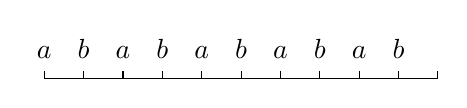
\begin{tikzpicture}

\sequenceeventtypes{0}{1em}{1}{1/a,2/b,3/a,4/b,5/a,6/b,7/a,8/b,9/a,10/b}
\sequencetickmarks{10}{0}{0}

\end{tikzpicture}
\end{center}

\end{frame}
\begin{frame}
\frametitle{Minimal windows}

$ \boldsymbol{s}[a, b) $ minimal window of $ \alpha $ if
\begin{itemize}
\item $ b - a \leq \rho $ for some $ \rho $
\item $ \boldsymbol{s}[a, b) \text{ covers } \alpha $
\item $ \nexists [c, d) \subset [a, b) : \boldsymbol{s} \text{ covers } \alpha $
\end{itemize}

\end{frame}
% TODO include this? maybe better show that minimal windows can overlap
\iffalse
\begin{frame}

\begin{center}
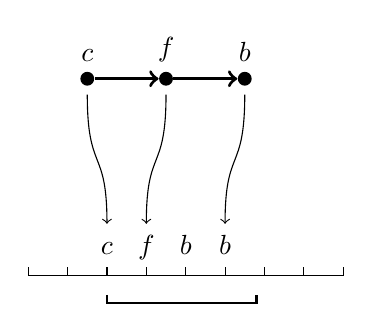
\begin{tikzpicture}

\sequencetickmarks{8}{-5.5}{0}
\sequenceeventtypes{-5.5}{1em}{30}{32/c,33/f,34/b,35/b}

\node (serC) at (-4.75,2.5) [smallnode,label={$ c $}] {};
\node (serF) at (-3.75,2.5) [smallnode,label={$ f $}] {};
\node (serB) at (-2.75,2.5) [smallnode,label={$ b $}] {};

\draw [->,very thick] (serC) -- (serF);
\draw [->,very thick] (serF) -- (serB);

\draw [->] ([yshift=-3pt]serC.south) .. controls +(0,-1) and +(0,1) .. (t32);
\draw [->] ([yshift=-3pt]serF.south) .. controls +(0,-1) and +(0,1) .. (t33);
\draw [->] ([yshift=-3pt]serB.south) .. controls +(0,-1) and +(0,1) .. (t35);

% windows

\windowthingy{(-4.5,-10pt)}{4}

\end{tikzpicture}
\end{center}

\end{frame}
\begin{frame}

\begin{center}
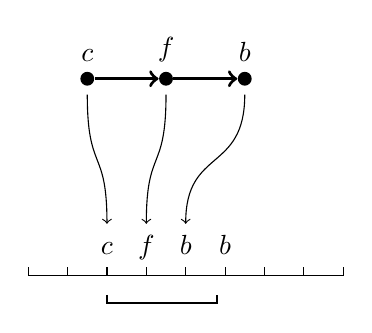
\begin{tikzpicture}

\sequencetickmarks{8}{-5.5}{0}
\sequenceeventtypes{-5.5}{1em}{30}{32/c,33/f,34/b,35/b}

\node (serC) at (-4.75,2.5) [smallnode,label={$ c $}] {};
\node (serF) at (-3.75,2.5) [smallnode,label={$ f $}] {};
\node (serB) at (-2.75,2.5) [smallnode,label={$ b $}] {};

\draw [->,very thick] (serC) -- (serF);
\draw [->,very thick] (serF) -- (serB);

\draw [->] ([yshift=-3pt]serC.south) .. controls +(0,-1) and +(0,1) .. (t32);
\draw [->] ([yshift=-3pt]serF.south) .. controls +(0,-1) and +(0,1) .. (t33);
\draw [->] ([yshift=-3pt]serB.south) .. controls +(0,-1) and +(0,1) .. (t34);

\windowthingy{(-4.5,-10pt)}{3}

\end{tikzpicture}
\end{center}

\end{frame}
\fi
\begin{frame}
episode $ \{ a, a, b \} $
\begin{center}
\footnotesize
\begin{tikzpicture}[scale=0.6]

\def\slidingwindowheight{0.5}
\def\interdotdistance{0.6}

\newcommand\letteratposition[1]
{\ifnum####1=2a\else\ifnum####1=3b\else\ifnum####1=5a\else\ifnum####1=7a\else0\fi\fi\fi\fi}

\newcommand\slidingwindowthingy[2]
{
    \foreach \i [evaluate=\i as \x using \i * \interdotdistance] in {0,...,7}
    {
        \ifnum\pdfstrcmp{\letteratposition{\i}}{0}=0
            \fill (\x,####1) circle [color=black,radius=2pt] node (n####2-\i) {};
        \else
            \draw (\x,####1) node [enoughdamnvspace, inner sep=1pt] (n####2-\i) {$ \letteratposition{\i} $};
        \fi
    }

    \node (dr####2) [right=7pt of n####2-7] {$ \cdots $};
}

\slidingwindowthingy{0}{0}
\draw (-0.5*\interdotdistance,-0.5*\slidingwindowheight) -- ++(2*\interdotdistance,0) -- ++(0,\slidingwindowheight) -- ++(-2*\interdotdistance,0);
\node (Qa) [right=1.5em of dr0,rotate=90,anchor=west,xshift=0.2cm] {$ Q(a) $};
\node (Qb) [right=4em of dr0,rotate=90,anchor=west,xshift=0.2cm] {$ Q(b) $};
\node (maxconsidera) [right=6em of dr0,rotate=90,anchor=west,xshift=0.2cm] {$ \text{maxcder}(\alpha, a) $};
\node (maxconsiderb) [right=7.5em of dr0,rotate=90,anchor=west,xshift=0.2cm] {$ \text{maxcder}(\alpha, b) $};

\node at (Qa |- dr0) {$ \langle \; \rangle $};
\node at (Qb |- dr0) {$ \langle \; \rangle $};
\node at (maxconsidera |- dr0) {$ 0 $};
\node at (maxconsiderb |- dr0) {$ 0 $};

\node at (n0-0 |- {(0,0.75)}) {\footnotesize $ 1 $};
\node at (n0-2 |- {(0,0.75)}) {\footnotesize $ 3 $};
\node at (n0-4 |- {(0,0.75)}) {\footnotesize $ 5 $};
\node at (n0-6 |- {(0,0.75)}) {\footnotesize $ 7 $};

\slidingwindowthingy{-1}{1}
\draw (-0.5*\interdotdistance,-1-0.5*\slidingwindowheight) -- ++(3*\interdotdistance,0) -- ++(0,\slidingwindowheight) -- ++(-3*\interdotdistance,0);

\node at (Qa |- dr1) {$ \langle 3 \rangle $};
\node at (Qb |- dr1) {$ \langle \; \rangle $};
\node at (maxconsidera |- dr1) {$ 1 $};
\node at (maxconsiderb |- dr1) {$ 0 $};

\slidingwindowthingy{-2}{2}
\draw (-0.5*\interdotdistance,-2-0.5*\slidingwindowheight) -- ++(4*\interdotdistance,0) -- ++(0,\slidingwindowheight) -- ++(-4*\interdotdistance,0);

\node at (Qa |- dr2) {$ \langle 3 \rangle $};
\node at (Qb |- dr2) {$ \langle 4 \rangle $};
\node at (maxconsidera |- dr2) {$ 1 $};
\node at (maxconsiderb |- dr2) {$ 1 $};

\slidingwindowthingy{-3}{3}
\draw (-0.5*\interdotdistance,-3-0.5*\slidingwindowheight) rectangle ++(6*\interdotdistance,\slidingwindowheight);

\node at (Qa |- dr3) {$ \langle 3, 6 \rangle $};
\node at (Qb |- dr3) {$ \langle 4 \rangle $};
\node at (maxconsidera |- dr3) {$ 2 $};
\node at (maxconsiderb |- dr3) {$ 1 $};

% \node [right=9em of dr3,align=left] {enough events in window\\and in consideration;\\minimal window found};

\draw ({(1.5*\interdotdistance,0)} |- n3-2.south) -- ++(0,-6pt) -- node (numwindowsindicator) [near start,below right,align=left] {determine minimal window} ++(4*\interdotdistance,0) -- ++(0,6pt);

\slidingwindowthingy{-5}{4}
\draw (0.5*\interdotdistance,-5-0.5*\slidingwindowheight) rectangle ++(6*\interdotdistance,\slidingwindowheight);

\node at (Qa |- dr4) {$ \langle 3, 6 \rangle $};
\node at (Qb |- dr4) {$ \langle 4 \rangle $};
\node at (maxconsidera |- dr4) {$ 1 $};
\node at (maxconsiderb |- dr4) {$ 1 $};

% \node [right=9em of dr4,align=left] {previous occurrence still in\\window, but first $ a $ out of \\ consideration};

\slidingwindowthingy{-6}{5}
\draw (1.5*\interdotdistance,-6-0.5*\slidingwindowheight) rectangle ++(6*\interdotdistance,\slidingwindowheight);

\node at (Qa |- dr5) {$ \langle 3, 6, 8 \rangle $};
\node at (Qb |- dr5) {$ \langle 4 \rangle $};
\node at (maxconsidera |- dr5) {$ 2 $};
\node at (maxconsiderb |- dr5) {$ 1 $};

% \node [right=9em of dr5,align=left] {new $ a $ entered; \\ another minimal window \\ found};

\draw ({(2.5*\interdotdistance,0)} |- n5-3.south) -- ++(0,-6pt) -- ++(5*\interdotdistance,0) -- ++(0,6pt);

\slidingwindowthingy{-7}{6}
\draw (7.5*\interdotdistance,-7-0.5*\slidingwindowheight) -- ++(-5*\interdotdistance,0) -- ++(0,\slidingwindowheight) -- ++(5*\interdotdistance,0);

\node at (Qa |- dr6) {$ \langle 6, 8 \rangle $};
\node at (Qb |- dr6) {$ \langle 4 \rangle $};
\node at (maxconsidera |- dr6) {$ 2 $};
\node at (maxconsiderb |- dr6) {$ 0 $};

\end{tikzpicture}
\end{center}

\end{frame}
\begin{frame}
\frametitle{Minimal-window frequency?}

$ fr_m(\alpha) = | mw(\alpha) | $ ?
\pause
\par\bigskip
Not monotonic!

\begin{center}
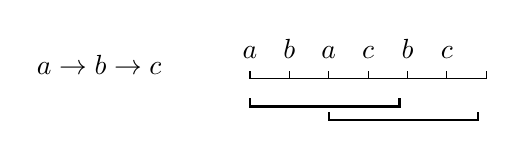
\begin{tikzpicture}
\sequencetickmarks{6}{0}{0}
\sequenceeventtypes{0}{1em}{1}{1/a,2/b,3/a,4/c,5/b,6/c}
\node at (-1,0.5em) [anchor=east] {$ a \to b \to c $};
\windowthingy{(0,-10pt)}{4}
\windowthingy{(1,-15pt)}{4}
\end{tikzpicture}
\end{center}
\begin{center}
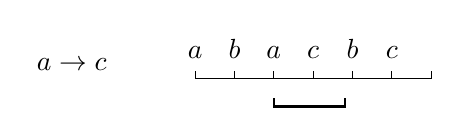
\begin{tikzpicture}
\sequencetickmarks{6}{0}{0}
\sequenceeventtypes{0}{1em}{1}{1/a,2/b,3/a,4/c,5/b,6/c}
\node at (-1,0.5em) [anchor=east] {$ a \to c $};
\windowthingy{(1,-10pt)}{2}
\end{tikzpicture}
\end{center}
% TODO maybe fix horizontal alignment of both pics (combine into one?)

\end{frame}
\begin{frame}
\frametitle{Disjoint-window frequency}

% Given window width $ \rho $, sequence $ \boldsymbol{s} $:
% \begin{align*}
% fr_m(\alpha) = \max\{ | W | \mid W \subseteq mw(\alpha) \wedge \forall ([a, b), [c, d)) \in W \times W \mid [a, b) \neq [c, d) : [a, b) \cup [c, d) = \emptyset \}
% \end{align*}
The disjoint-window frequency is defined as the maximal number of non-overlapping minimal windows.

\begin{align*}
fr_m(\alpha) = \max\{ | W | \mid W \subseteq mw(\alpha) \wedge dis(W) \}
\end{align*}

\end{frame}
\begin{frame}

episode $ \{ a, b \} $

\begin{center}
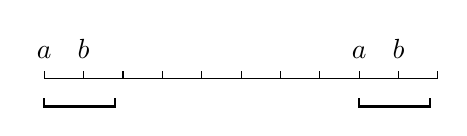
\begin{tikzpicture}

\sequenceeventtypes{0}{1em}{1}{1/a,2/b,9/a,10/b}
\sequencetickmarks{10}{0}{0}

\windowthingy{(0,-10pt)}{2}
\windowthingy{(4,-10pt)}{2}

\end{tikzpicture}

\par\bigskip

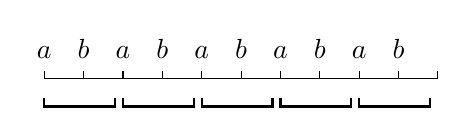
\begin{tikzpicture}

\sequenceeventtypes{0}{1em}{1}{1/a,2/b,3/a,4/b,5/a,6/b,7/a,8/b,9/a,10/b}
\sequencetickmarks{10}{0}{0}

\windowthingy{(0,-10pt)}{2}
\windowthingy{(1,-10pt)}{2}
\windowthingy{(2,-10pt)}{2}
\windowthingy{(3,-10pt)}{2}
\windowthingy{(4,-10pt)}{2}

\end{tikzpicture}
\end{center}

\end{frame}
\begin{frame}
\begin{center}
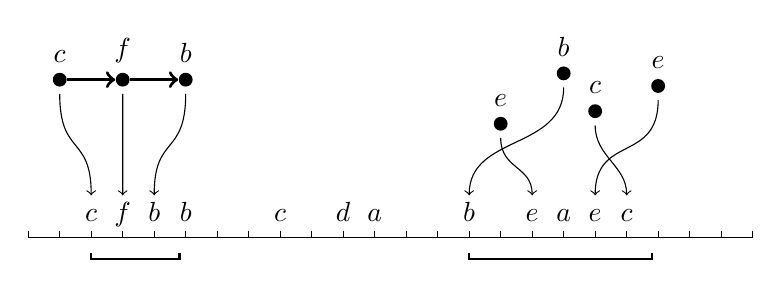
\begin{tikzpicture}[scale=0.8]

\examplesequence

%% draw occurrence proofs again
% serial episode

\node (serC) at (-5,2.5) [smallnode,label={$ c $}] {};
\node (serF) at (-4,2.5) [smallnode,label={$ f $}] {};
\node (serB) at (-3,2.5) [smallnode,label={$ b $}] {};

\draw [->,very thick] (serC) -- (serF);
\draw [->,very thick] (serF) -- (serB);

\draw [->] ([yshift=-3pt]serC.south) .. controls +(0,-1) and +(0,1) .. (t32);
\draw [->] ([yshift=-3pt]serF.south) .. controls +(0,-1) and +(0,1) .. (t33);
\draw [->] ([yshift=-3pt]serB.south) .. controls +(0,-1) and +(0,1) .. (t34);

% parallel episode

\node (parB) at (3,2.6) [smallnode,label={$ b $}] {};
\node (parE1) at (2,1.8) [smallnode,label={$ e $}] {};
\node (parE2) at (4.5,2.4) [smallnode,label={$ e $}] {};
\node (parC) at (3.5,2) [smallnode,label={$ c $}] {};

\draw [->] ([yshift=-3pt]parB.south) .. controls +(0,-1) and +(0,1) .. (t44);
\draw [->] ([yshift=-3pt]parE1.south) .. controls +(0,-0.5) and +(0,0.5) .. (t46);
\draw [->] ([yshift=-3pt]parE2.south) .. controls +(0,-1) and +(0,1) .. (t48);
\draw [->] ([yshift=-3pt]parC.south) .. controls +(0,-0.5) and +(0,0.5) .. (t49);

% windows

\windowthingy{(-4.5,-10pt)}{3}

\windowthingy{(1.5,-10pt)}{6}

\end{tikzpicture}
\end{center}
\end{frame}
\begin{frame}
\frametitle{Weighted-window frequency}

The weighted-window frequency is defined as the sum of weights of the set of windows that maximizes this sum.

\begin{align*}
fr_w(\alpha) = \max \left\{ \sum_{[a, b) \in W}{\frac{1}{b - a}} \,\middle\vert\, W \subseteq mw(\alpha) \wedge dis(W) \right \}
\end{align*}

\end{frame}
\begin{frame}
\begin{center}
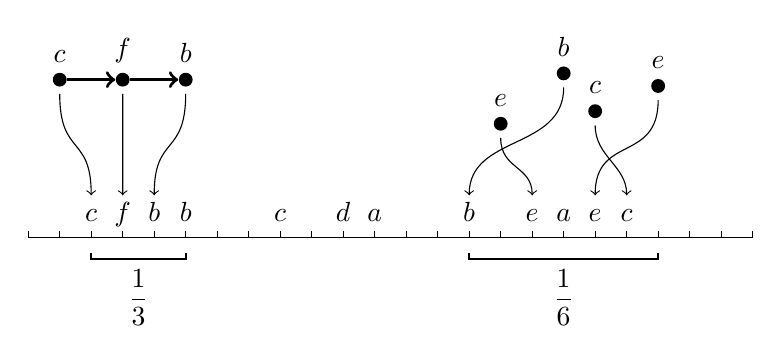
\begin{tikzpicture}[scale=0.8]

\examplesequence

%% draw occurrence proofs again
% serial episode

\node (serC) at (-5,2.5) [smallnode,label={$ c $}] {};
\node (serF) at (-4,2.5) [smallnode,label={$ f $}] {};
\node (serB) at (-3,2.5) [smallnode,label={$ b $}] {};

\draw [->,very thick] (serC) -- (serF);
\draw [->,very thick] (serF) -- (serB);

\draw [->] ([yshift=-3pt]serC.south) .. controls +(0,-1) and +(0,1) .. (t32);
\draw [->] ([yshift=-3pt]serF.south) .. controls +(0,-1) and +(0,1) .. (t33);
\draw [->] ([yshift=-3pt]serB.south) .. controls +(0,-1) and +(0,1) .. (t34);

% parallel episode

\node (parB) at (3,2.6) [smallnode,label={$ b $}] {};
\node (parE1) at (2,1.8) [smallnode,label={$ e $}] {};
\node (parE2) at (4.5,2.4) [smallnode,label={$ e $}] {};
\node (parC) at (3.5,2) [smallnode,label={$ c $}] {};

\draw [->] ([yshift=-3pt]parB.south) .. controls +(0,-1) and +(0,1) .. (t44);
\draw [->] ([yshift=-3pt]parE1.south) .. controls +(0,-0.5) and +(0,0.5) .. (t46);
\draw [->] ([yshift=-3pt]parE2.south) .. controls +(0,-1) and +(0,1) .. (t48);
\draw [->] ([yshift=-3pt]parC.south) .. controls +(0,-0.5) and +(0,0.5) .. (t49);

% windows

\draw [thick] (-4.5,-7pt) -- ++(0,-3pt) -- ++(1.5,0) node [midway,below] {$ \dfrac13 $} -- ++(0,3pt);

\draw [thick] (1.5,-7pt) -- ++(0,-3pt) -- ++(3,0) node [midway,below] {$ \dfrac16 $} -- ++(0,3pt);

\end{tikzpicture}
\end{center}
\end{frame}
\begin{frame}
\frametitle{Association rules}

Given episodes $ \alpha \subset \beta $, we can express association rule $ \alpha \Rightarrow \beta $.
\par\bigskip
Confidence $ c(\alpha \Rightarrow \beta) $ expresses likelihood of finding $ \beta $, given occurrence of $ \alpha $.

\end{frame}
\begin{frame}
\frametitle{Fixed-window confidence}

\begin{align*}
c_f(\alpha \Rightarrow \beta) = \frac{ fr_f(\beta) }{ fr_f(\alpha) }
\end{align*}

Expresses the probability of $ \beta $ occurring in a window which covers $ \alpha $.

\end{frame}
\begin{frame}
\frametitle{Minimal-window confidence?}

Naive approach, analogous to fixed-window confidence:
\begin{align*}
c_m(\alpha \Rightarrow \beta) = \frac{| fr_m(\beta) |}{| fr_m(\alpha) |}
\end{align*}
\pause
\par\bigskip
But then\begin{align*}c_m(\{ a \} \Rightarrow \{ a, a \}) \leq \frac12 \end{align*} in sequence $ \cdots\;a\;a\;\cdots\;a\;a\cdots\;a\,a\cdots $



\end{frame}
\begin{frame}
\frametitle{Minimal-window confidence}

The minimal-window confidence is defined as the percentage of minimal windows of $ \alpha $ that are contained within a minimal window of $ \beta $.

\begin{align*}
ext_m(\boldsymbol{s}[a, b), \alpha, \beta) =
\begin{cases}
    1 & \text{ if } \exists [c, d) \in mw(\beta) \mid [a, b) \subset [c, d) \\
    0 & \text{ otherwise}
\end{cases}
\end{align*}
\begin{align*}
c_m(\alpha \Rightarrow \beta) = \frac{\sum_{w \in mw(\alpha)} ext_m(w, \alpha, \beta)}{| mw(\alpha) |}
\end{align*}

\end{frame}
\begin{frame}
\frametitle{Weighted-window confidence}

Inverse of weighted-extensibility expresses how far $ [a, b) $ needs to be extended in order to find occurrence of $ \beta $.
\begin{align*}
ext_w(\boldsymbol{s}[a, b), \alpha, \beta) = \frac{b - a}{d - c}
\end{align*}

\begin{align*}
c_w(\alpha \Rightarrow \beta) = \frac{\sum_{w \in mw(\alpha)} ext_w(w, \alpha, \beta)}{| mw(\alpha) |}
\end{align*}

\end{frame}
\begin{frame}
\begin{center}
\begin{tikzpicture}[scale=0.8]

\examplesequence

% parallel episode

\node (parB) at (3,2.6) [smallnode,label={$ b $}] {};
\node (parE1) at (2,1.8) [smallnode,label={$ e $}] {};
\node (parE2) at (4.5,2.4) [smallnode,label={$ e $}] {};
\node (parC) at (3.5,2) [smallnode,label={$ c $}] {};

\draw [->] ([yshift=-3pt]parB.south) .. controls +(0,-1) and +(0,1) .. (t44);
\draw [->] ([yshift=-3pt]parE1.south) .. controls +(0,-0.5) and +(0,0.5) .. (t46);
\draw [->] ([yshift=-3pt]parE2.south) .. controls +(0,-1) and +(0,1) .. (t48);
\draw [->] ([yshift=-3pt]parC.south) .. controls +(0,-0.5) and +(0,0.5) .. (t49);

\end{tikzpicture}
\end{center}
\begin{center}
\begin{tabulary}{\textwidth}{L|S|S|S}
& $ c_f $ & $ c_m $ & $ c_w $ \\
\hline
$ \{ b \}    \Rightarrow \{ b, c, e, e \} $ & 0.18 & 0.33 & 0.056 \\
$ \{ c \}    \Rightarrow \{ b, c, e, e \} $ & 0.14 & 0.33 & 0.056 \\
$ \{ b, c \} \Rightarrow \{ b, c, e, e \} $ & 0.21 & 0.25 & 0.25 \\
$ \{ e \}    \Rightarrow \{ b, c, e, e \} $ & 0.3  & 1    & 0.17 \\
$ \{ c, e \} \Rightarrow \{ b, c, e, e \} $ & 0.43 & 1    & 0.33 \\
$ \{ e, e \} \Rightarrow \{ b, c, e, e \} $ & 0.5  & 1    & 0.5 \\
$ \{ b, e \} \Rightarrow \{ b, c, e, e \} $ & 0.5  & 1    & 0.5 \\
\end{tabulary}
\end{center}
\end{frame}
\begin{frame}
\frametitle{Experiments}

\begin{center}
\begin{tabulary}{\textwidth}{ L|RRRC }
dataset & \multicolumn{1}{c}{$ | \Sigma | $} & \multicolumn{1}{c}{$ | s | $} & \multicolumn{1}{c}{$ T_e - T_s $} & type \\
\hline
\emph{abstract} & \num{51.3d3} & \num{67.8d3} & \num{67.8d3} & dense \\
\emph{tolstoy} & \num{95.6d3} & \num{124d3} & \num{124d3} & dense \\
\emph{trains} & \num{1.28d3} & \num{10.1d3} & \num{2.67d6} & sparse \\
\end{tabulary}
\par\bigskip
\begin{tikzpicture}[scale=0.5]

\begin{axis}[
    xlabel={event types ordered by frequency},
    ylabel={number of occurrences},
    xmin=-100,
    ymin=-50,
    % ymode=log
]

\addplot table [x=rank,y=count,mark=none] {experiments/tolstoy-alphabet-frequency-2200.dat};

\end{axis}

\end{tikzpicture}
\qquad
\begin{tikzpicture}[scale=0.5]

\begin{axis}[
    xlabel={event types ordered by frequency},
    ylabel={number of occurrences},
    xmin=-50,
    ymin=-1,
    % ymode=log
]

\addplot table [x=rank,y=count,mark=none] {experiments/trains-alphabet-frequency.tsv};

\end{axis}

\end{tikzpicture}
\end{center}

\end{frame}
\begin{frame}
\frametitle{Cumulative distribution \emph{trains}}

\begin{center}
\begin{tikzpicture}[scale=0.5]

\begin{axis}[
    xlabel={timestamp},
    ylabel={cumulative events},
    % xmin=-10,
    % ymin=-50,
    % ymode=log
]

\addplot table [x=time,y=count,mark=none] {experiments/trains-cumulative.dat};

\end{axis}

\end{tikzpicture}
\qquad
\begin{tikzpicture}[scale=0.5]

\begin{axis}[
    xlabel={timestamp},
    ylabel={cumulative events},
    % xmin=-10,
    % ymin=-50,
    % ymode=log
]

\addplot table [x=time,y=count,mark=none] {experiments/trains-cumulative-part.dat};

\end{axis}

\end{tikzpicture}

\end{center}
\end{frame}
\begin{frame}
\begingroup\footnotesize
\begin{tabulary}{\textwidth}{R|L|L|L}%
\# & fixed-window fr. & disjoint-window fr. & weighted-window fr. \\
\hline
1 & $ \{ \text{levin} \} $ (20913) & $ \{ \text{levin} \} $ (1629) & $ \{ \text{levin} \} $ (1629) \\
2 & $ \{ \text{vronski} \} $ (11165) & $ \{ \text{vronski} \} $ (865) & $ \{ \text{vronski} \} $ (865) \\
3 & $ \{ \text{anna} \} $ (10699) & $ \{ \text{anna} \} $ (823) & $ \{ \text{anna} \} $ (823) \\
4 & $ \{ \text{thought} \} $ (8994) & $ \{ \text{kitti} \} $ (672) & $ \{ \text{kitti} \} $ (672) \\
5 & $ \{ \text{time} \} $ (8948) & $ \{ \text{thought} \} $ (663) & $ \{ \text{thought} \} $ (663) \\
6 & $ \{ \text{kitti} \} $ (8826) & $ \{ \text{time} \} $ (651) & $ \{ \text{time} \} $ (651) \\
7 & $ \{ \text{hand} \} $ (8645) & $ \{ \text{hand} \} $ (651) & $ \{ \text{hand} \} $ (651) \\
8 & $ \{ \text{alexei} \} $ (8619) & $ \{ \text{smile} \} $ (632) & $ \{ \text{smile} \} $ (632) \\
9 & $ \{ \text{smile} \} $ (8549) & $ \{ \text{alexei} \} $ (632) & $ \{ \text{alexei} \} $ (632) \\
10 & $ \{ \text{face} \} $ (8315) & $ \{ \text{face} \} $ (598) & $ \{ \text{face} \} $ (598) \\
11 & $ \{ \text{ey} \} $ (8062) & $ \{ \text{love} \} $ (595) & $ \{ \text{love} \} $ (595) \\
12 & $ \{ \text{alexandrovitch} \} $ (7842) & $ \{ \text{alexandrovitch} \} $ (571) & $ \{ \text{alexandrovitch} \} $ (571) \\
13 & $ \{ \text{felt} \} $ (7753) & $ \{ \text{alexei},\allowbreak\text{alexandrovitch} \} $ (571) & $ \{ \text{ey} \} $ (570) \\
14 & $ \{ \text{man} \} $ (7751) & $ \{ \text{ey} \} $ (570) & $ \{ \text{man} \} $ (565) \\
15 & $ \{ \text{feel} \} $ (7596) & $ \{ \text{man} \} $ (565) & $ \{ \text{feel} \} $ (561) \\
\end{tabulary}%
\endgroup

\end{frame}
\begin{frame}

\begin{center}
\begingroup\footnotesize
\begin{tabulary}{\textwidth}{R|L}
\# & fixed-window fr. \\
\hline
1 & $ \{ \text{alexei},\allowbreak\text{alexandrovitch} \} $ (7416) \\
2 & $ \{ \text{stepan},\allowbreak\text{arkadyevitch} \} $ (7117) \\
3 & $ \{ \text{sergei},\allowbreak\text{ivanovitch} \} $ (3763) \\
4 & $ \{ \text{levin},\allowbreak\text{levin} \} $ (3348) \\
5 & $ \{ \text{darya},\allowbreak\text{alexandrovna} \} $ (2739) \\
6 & $ \{ \text{levin},\allowbreak\text{kitti} \} $ (2039) \\
7 & $ \{ \text{anna},\allowbreak\text{vronski} \} $ (1942) \\
8 & $ \{ \text{arkadyevitch},\allowbreak\text{levin} \} $ (1896) \\
9 & $ \{ \text{stepan},\allowbreak\text{levin} \} $ (1887) \\
10 & $ \{ \text{stepan},\allowbreak\text{arkadyevitch},\allowbreak\text{levin} \} $ (1784) \\
11 & $ \{ \text{smile},\allowbreak\text{levin} \} $ (1778) \\
12 & $ \{ \text{vronski},\allowbreak\text{vronski} \} $ (1722) \\
13 & $ \{ \text{time},\allowbreak\text{levin} \} $ (1597) \\
14 & $ \{ \text{brother},\allowbreak\text{levin} \} $ (1558) \\
15 & $ \{ \text{anna},\allowbreak\text{anna} \} $ (1531) \\
\end{tabulary}%
\endgroup
\end{center}

\end{frame}
\begin{frame}

\begin{center}
\begingroup\footnotesize
\begin{tabulary}{\textwidth}{R|L}
\# & disjoint-window fr. \\
\hline
1 &  $ \{ \text{alexei},\allowbreak\text{alexandrovitch} \} $ (571) \\
2 &  $ \{ \text{stepan},\allowbreak\text{arkadyevitch} \} $ (547) \\
3 &  $ \{ \text{levin},\allowbreak\text{levin} \} $ (395) \\
4 &  $ \{ \text{sergei},\allowbreak\text{ivanovitch} \} $ (291) \\
5 &  $ \{ \text{darya},\allowbreak\text{alexandrovna} \} $ (205) \\
6 &  $ \{ \text{levin},\allowbreak\text{kitti} \} $ (202) \\
7 &  $ \{ \text{stepan},\allowbreak\text{levin} \} $ (199) \\
8 &  $ \{ \text{arkadyevitch},\allowbreak\text{levin} \} $ (197) \\
9 &  $ \{ \text{stepan},\allowbreak\text{arkadyevitch},\allowbreak\text{levin} \} $ (195) \\
10 & $ \{ \text{vronski},\allowbreak\text{vronski} \} $ (191) \\
11 & $ \{ \text{anna},\allowbreak\text{vronski} \} $ (180) \\
12 & $ \{ \text{smile},\allowbreak\text{levin} \} $ (171) \\
13 & $ \{ \text{anna},\allowbreak\text{anna} \} $ (170) \\
14 & $ \{ \text{time},\allowbreak\text{levin} \} $ (159) \\
15 & $ \{ \text{good},\allowbreak\text{levin} \} $ (153) \\
\end{tabulary}%
\endgroup
\end{center}

\end{frame}
\begin{frame}

\begin{center}
\begingroup\footnotesize
\begin{tabulary}{\textwidth}{R|L}
\# & weighted-window fr. \\
\hline
1 & $ \{ \text{alexei},\allowbreak\text{alexandrovitch} \} $ (286) \\
2 & $ \{ \text{stepan},\allowbreak\text{arkadyevitch} \} $ (274) \\
3 & $ \{ \text{sergei},\allowbreak\text{ivanovitch} \} $ (146) \\
4 & $ \{ \text{darya},\allowbreak\text{alexandrovna} \} $ (102) \\
5 & $ \{ \text{levin},\allowbreak\text{levin} \} $ (61.6) \\
6 & $ \{ \text{lidia},\allowbreak\text{ivanovna} \} $ (54) \\
7 & $ \{ \text{anna},\allowbreak\text{vronski} \} $ (45.1) \\
8 & $ \{ \text{smile},\allowbreak\text{levin} \} $ (41.3) \\
9 & $ \{ \text{levin},\allowbreak\text{kitti} \} $ (41.1) \\
10& $ \{ \text{room},\allowbreak\text{draw} \} $ (40.6) \\
11& $ \{ \text{countess},\allowbreak\text{lidia} \} $ (39.4) \\
12& $ \{ \text{thought},\allowbreak\text{levin} \} $ (39.3) \\
13& $ \{ \text{love},\allowbreak\text{love} \} $ (38.2) \\
14& $ \{ \text{arkadyevitch},\allowbreak\text{levin} \} $ (37.2) \\
15& $ \{ \text{agafea},\allowbreak\text{mihalovna} \} $ (37) \\
\end{tabulary}%
\endgroup
\end{center}

\end{frame}
\begin{frame}
\frametitle{Cohesion-based measures}

Mean-based cohesion:
\begin{align*}
C(\alpha) = \frac{| \alpha |}{\overline{W}(\alpha)}
\end{align*}
\par\bigskip
Quantile-based cohesion:
\begin{align*}
C_q(\alpha) = \frac{| \{ t \mid t \in \text{cover}(\alpha) \wedge W_t(\alpha) < \rho \cdot | \alpha | \} |}{\text{support}(\alpha)}
\end{align*}

\end{frame}
\begin{frame}
\footnotesize
\begin{center}
\begin{tabulary}{\textwidth}{R|L|L}

\# & mean-based cohesion & quantile-based cohesion \\
\hline
1 & $ \{ \text{agafea}, \text{mihalovna} \} $ (1) & $ \text{stepan} \to \text{arkadyevitch} $ (0.998) \\
2 & $ \{ \text{char}, \text{banc} \} $ (1) & $ \text{alexei} \to \text{alexandrovitch} $ (0.95) \\
3 & $ \{ \text{pinc}, \text{nez} \} $ (1) & $ \text{sergei} \to \text{ivanovitch} $ (0.965) \\
4 & $ \{ \text{bell}, \text{soeur} \} $ (1) & $ \text{agafea} \to \text{mihalovna} $ (1, 148) \\
5 & $ \{ \text{stepan}, \text{arkadyevitch} \} $ (0.915) & $ \text{darya} \to \text{alexandrovna} $ (0.967) \\
6 & $ \{ \text{nativ}, \text{tribe} \} $ (0.523) & $ \text{char} \to \text{banc} $ (1) \\
7 & $ \{ \text{lizaveta}, \text{petrovna} \} $ (0.408) & $ \text{pinc} \to \text{nez} $ (1) \\
8 & $ \{ \text{ivanovna}, \text{lidia} \} $ (0.137) & $ \text{bell} \to \text{soeur} $ (1) \\
9 & $ \{ \text{alexandrovitch}, \text{alexei} \} $ (0.05) & $ \text{lidia} \to \text{ivanovna} $ (0.977) \\
10 & $ \{ \text{sergei}, \text{ivanovitch} \} $ (0.0428) & $ \text{lizaveta} \to \text{petrovna} $ (0.98) \\
11 & $ \{ \text{darya}, \text{alexandrovna} \} $ (0.0363) & $ \text{nativ} \to \text{tribe} $ (0.966) \\
12 & $ \{ \text{bezzubov}, \text{landau} \} $ (0.0351) & $ \text{mashkin} \to \text{upland} $ (0.833) \\
13 & $ \{ \text{gladiat}, \text{frou} \} $ (0.0326) & $ \text{grand} \to \text{duchess} $ (0.714) \\
14 & $ \{ \text{partnership}, \text{ryezunov} \} $ (0.0303) & $ \text{liza} \to \text{merkalova} $ (0.706) \\
15 & $ \{ \text{bridal}, \text{lectern} \} $ (0.0281) & $ \text{marya} \to \text{nikolaevna} $ (0.673) \\
\end{tabulary}
\end{center}

\end{frame}
\begin{frame}
\footnotesize
\begin{center}
\begin{tabulary}{\textwidth}{R|L}
\# & mean-based cohesion (cohesion) \\
\hline
40 & $ \{ \text{ey},\allowbreak \text{face},\allowbreak \text{smile},\allowbreak \text{hand} \} $ (0.0164) \\
41 & $ \{ \text{feel},\allowbreak \text{ey},\allowbreak \text{face},\allowbreak \text{smile},\allowbreak \text{hand} \} $ (0.0164) \\
42 & $ \{ \text{feel},\allowbreak \text{ey},\allowbreak \text{smile},\allowbreak \text{time},\allowbreak \text{hand} \} $ (0.0161) \\
43 & $ \{ \text{ey},\allowbreak \text{smile},\allowbreak \text{time},\allowbreak \text{hand},\allowbreak \text{thought} \} $ (0.0161) \\
44 & $ \{ \text{chapter},\allowbreak \text{ey},\allowbreak \text{smile},\allowbreak \text{time},\allowbreak \text{hand} \} $ (0.0161) \\
45 & $ \{ \text{chapter},\allowbreak \text{felt},\allowbreak \text{feel},\allowbreak \text{time},\allowbreak \text{thought} \} $ (0.0161) \\
46 & $ \{ \text{chapter},\allowbreak \text{face},\allowbreak \text{smile},\allowbreak \text{time},\allowbreak \text{hand} \} $ (0.016) \\
47 & $ \{ \text{troth},\allowbreak \text{bridal} \} $ (0.016) \\
48 & $ \{ \text{ey},\allowbreak \text{smile},\allowbreak \text{hand} \} $ (0.016) \\
49 & $ \{ \text{face},\allowbreak \text{smile},\allowbreak \text{hand} \} $ (0.0159) \\
\end{tabulary}
\end{center}

\end{frame}
\begin{frame}
\footnotesize
\begin{center}
\begin{tabulary}{\textwidth}{R|L}
\# & quantile-based cohesion (cohesion, support) \\
\hline
27 & $ \text{bridal} \to \text{pair} $ (0.5, 20) \\
45 & $ \text{wag} \to \text{tail} $ (0.4, 20) \\
46 & $ \text{unbutton} \to \text{waistcoat} $ (0.3, 20) \\
62 & $ \text{lightn} \to \text{thunder} $ (0.364, 11) \\
67 & $ \text{hall} \to \text{porter} $ (0.344, 128) \\
91 & $ \text{hawk} \to \text{hover} $ (0.308, 13) \\
84 & $ \text{district} \to \text{council} $ (0.325, 77) \\
110 & $ \text{butter} \to \text{salt} $ (0.294, 17) \\
116 & $ \text{lime} \to \text{tree} $ (0.282, 71) \\
122 & $ \text{summer} \to \text{villa} $ (0.281, 64) \\
131 & $ \text{carpent} \to \text{harrow} \to \text{repair} $ (0.25, 32) \\
\end{tabulary}
\end{center}

\end{frame}
\begin{frame}
\frametitle{Performance: runtimes \emph{abstract}}

\begin{figure}

\begin{subfigure}[b]{0.5\textwidth}
\centering

\begin{tikzpicture}[scale=0.6]

\begin{axis}[
    legend entries={fixed windows,minimal windows,weighted windows},
    legend style={legend pos=south east},
    xlabel={number of frequent episodes},
    ylabel={runtime (s)},
    xmode=log,
    ymode=log,
]

\addplot table [x=num-frequent-episodes,y=duration-s] {experiments/nsf/nsf-parallel-fixed-windows-15.tsv};
\addplot table [x=num-frequent-episodes,y=duration-s] {experiments/nsf/nsf-parallel-minimal-windows-15.tsv};
\addplot table [x=num-frequent-episodes,y=duration-s] {experiments/nsf/nsf-parallel-weighted-windows-15.tsv};

\end{axis}

\end{tikzpicture}

\caption{parallel episodes}
\end{subfigure}%
\begin{subfigure}[b]{0.5\textwidth}
\centering

\begin{tikzpicture}[scale=0.6]

\begin{axis}[
    legend entries={fixed windows,minimal windows,weighted windows},
    legend style={legend pos=south east},
    xlabel={number of frequent episodes},
    ylabel={runtime (s)},
    xmode=log,
    ymode=log,
]

\addplot table [x=num-frequent-episodes,y=duration-s] {experiments/nsf/nsf-serial-fixed-windows-15.tsv};
\addplot table [x=num-frequent-episodes,y=duration-s] {experiments/nsf/nsf-serial-minimal-windows-15.tsv};
\addplot table [x=num-frequent-episodes,y=duration-s] {experiments/nsf/nsf-serial-weighted-windows-15.tsv};

\end{axis}

\end{tikzpicture}

\caption{serial episodes}
\end{subfigure}

\label{fig:runtimes-nsf-15}
\end{figure}

\end{frame}
\begin{frame}
\frametitle{Performance: runtimes \emph{tolstoy}}

\begin{figure}

\begin{subfigure}[b]{0.5\textwidth}
\centering

\begin{tikzpicture}[scale=0.6]

\begin{axis}[
    legend entries={fixed windows,minimal windows,weighted windows},
    legend style={legend pos=south east},
    xlabel={number of frequent episodes},
    ylabel={runtime (s)},
    xmode=log,
    ymode=log,
]

\addplot table [x=num-frequent-episodes,y=duration-s] {experiments/tolstoy/tolstoy-parallel-fixed-windows-15.tsv};
\addplot table [x=num-frequent-episodes,y=duration-s] {experiments/tolstoy/tolstoy-parallel-minimal-windows-15.tsv};
\addplot table [x=num-frequent-episodes,y=duration-s] {experiments/tolstoy/tolstoy-parallel-weighted-windows-15.tsv};

\end{axis}

\end{tikzpicture}

\caption{parallel episodes}
\end{subfigure}%
\begin{subfigure}[b]{0.5\textwidth}
\centering

\begin{tikzpicture}[scale=0.6]

\begin{axis}[
    legend entries={fixed windows,minimal windows,weighted windows},
    legend style={legend pos=north west},
    xlabel={number of frequent episodes},
    ylabel={runtime (s)},
    xmode=log,
    ymode=log,
]

\addplot table [x=num-frequent-episodes,y=duration-s] {experiments/tolstoy/tolstoy-serial-fixed-windows-15.tsv};
\addplot table [x=num-frequent-episodes,y=duration-s] {experiments/tolstoy/tolstoy-serial-minimal-windows-15.tsv};
\addplot table [x=num-frequent-episodes,y=duration-s] {experiments/tolstoy/tolstoy-serial-weighted-windows-15.tsv};

\end{axis}

\end{tikzpicture}

\caption{serial episodes}
\end{subfigure}

\label{fig:runtimes-tolstoy-15}
\end{figure}

\end{frame}
\begin{frame}
\frametitle{Performance: runtimes \emph{trains}}

\begin{figure}

\begin{subfigure}[b]{0.5\textwidth}
\centering

\begin{tikzpicture}[scale=0.6]

\begin{axis}[
    legend entries={fixed windows,minimal windows,weighted windows},
    legend style={legend pos=south east},
    xlabel={number of frequent episodes},
    ylabel={runtime (s)},
    xmode=log,
    ymode=log,
]

\addplot table [x=num-frequent-episodes,y=duration-s] {experiments/trains/trains-parallel-fixed-windows-900.tsv};
\addplot table [x=num-frequent-episodes,y=duration-s] {experiments/trains/trains-parallel-minimal-windows-900.tsv};
\addplot table [x=num-frequent-episodes,y=duration-s] {experiments/trains/trains-parallel-weighted-windows-900.tsv};

\end{axis}

\end{tikzpicture}

\caption{parallel episodes}
\label{fig:runtimes-trains-900-parallel}
\end{subfigure}%
\begin{subfigure}[b]{0.5\textwidth}
\centering

\begin{tikzpicture}[scale=0.6]

\begin{axis}[
    legend entries={fixed windows,minimal windows,weighted windows},
    legend style={legend pos=south east},
    xlabel={number of frequent episodes},
    ylabel={runtime (s)},
    xmode=log,
    ymode=log,
]

\addplot table [x=num-frequent-episodes,y=duration-s] {experiments/trains/trains-serial-fixed-windows-900.tsv};
\addplot table [x=num-frequent-episodes,y=duration-s] {experiments/trains/trains-serial-minimal-windows-900.tsv};
\addplot table [x=num-frequent-episodes,y=duration-s] {experiments/trains/trains-serial-weighted-windows-900.tsv};

\end{axis}

\end{tikzpicture}

\caption{serial episodes}
\label{fig:runtimes-trains-900-serial}
\end{subfigure}

\label{fig:runtimes-trains-900}
\end{figure}

\end{frame}
\begin{frame}

\begin{figure}
\begin{subfigure}[t]{0.48\textwidth}
\centering
\begin{tikzpicture}[scale=0.6]

\begin{axis}[
    legend entries={parallel episodes,serial episodes},
    legend style={legend pos=south west},
    xlabel={frequency threshold},
    ylabel={runtime (s)},
    xmode=log,
    ymode=log,
    % x dir=reverse,
]

\addplot table [x=frequency-threshold,y=duration-s] {experiments/trains/trains-parallel-weighted-windows-900.tsv};
\addplot table [x=frequency-threshold,y=duration-s] {experiments/trains/trains-serial-weighted-windows-900.tsv};

\end{axis}

\end{tikzpicture}
\caption{Runtime as a function of the frequency threshold.}
\label{fig:investigate-trains-runtimes-runtimes}
\end{subfigure}%
\hfill%
\begin{subfigure}[t]{0.48\textwidth}
\begin{tikzpicture}[scale=0.6]

\begin{axis}[
    legend entries={1-episodes,2-episodes,3-episodes,4-episodes,5-episodes,6-episodes,7-episodes,8-episodes,9-episodes,10-episodes,11-episodes,12-episodes,13-episodes,14-episodes,15-episodes},
    legend style={legend pos=north east,legend style={nodes={scale=0.75}}},
    xlabel={frequency threshold},
    ylabel={number of frequent $ l $-episodes},
    xmode=log,
    ymode=log,
]

\addplot table [x=frequency-threshold,y=num-frequent-1-episodes] {experiments/trains/trains-parallel-weighted-windows-900.tsv};
\addplot table [x=frequency-threshold,y=num-frequent-2-episodes] {experiments/trains/trains-parallel-weighted-windows-900.tsv};
\addplot table [x=frequency-threshold,y=num-frequent-3-episodes] {experiments/trains/trains-parallel-weighted-windows-900.tsv};
\addplot table [x=frequency-threshold,y=num-frequent-4-episodes] {experiments/trains/trains-parallel-weighted-windows-900.tsv};
\addplot table [x=frequency-threshold,y=num-frequent-5-episodes] {experiments/trains/trains-parallel-weighted-windows-900.tsv};

\end{axis}
\end{tikzpicture}
\caption{Number of frequent parallel $ l $-episodes as a function of the frequency threshold.}
\label{fig:investigate-trains-runtimes-frequencies}
\end{subfigure}
\label{fig:investigate-trains-runtimes}
\end{figure}

\end{frame}
\begin{frame}
\frametitle{Conclusion}

\begin{itemize}
\item<1-> Were able to find interesting patterns.
\item<2-> All interestingness measures have advantages and disadvantages.
\item<3-> Both frequency-based and cohesion-based frequency measures have their merit.
\item<4-> More redundancy elimination would be welcome.
\end{itemize}

\end{frame}

\end{document}
